\section*{Appendix}
\addcontentsline{toc}{section}{Appendix}

\subsection{Web-Based Platform for Data Partitioning Evaluation}\label{subsec:web_platform}

\begin{figure*}
    \centering
    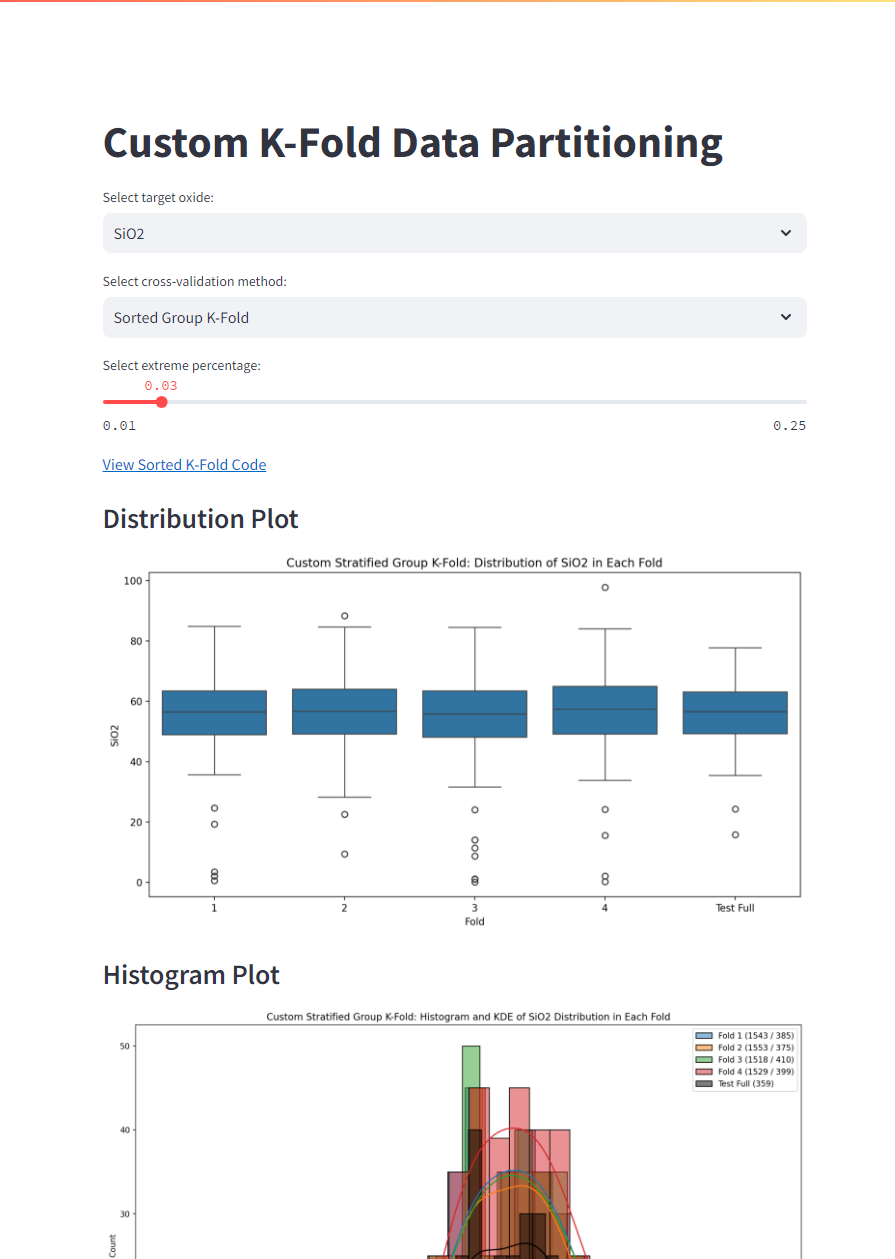
\includegraphics[width=0.7\textwidth]{images/web_platform.png}
    \caption{Web-based platform used to determine the optimal value of $p$ for the data partitioning algorithm.}
    \label{fig:web_platform}
\end{figure*}

\FloatBarrier

\subsection{Cross-Validation Fold Plots for Major Oxides}\label{subsec:cv_plots}

% Loop through each major oxide and add a subsubsection with figures
\foreach \oxide in {SiO2, TiO2, Al2O3, FeOT, MgO, CaO, Na2O, K2O} {
    \subsubsection{\oxide}

    \begin{figure*}
        \centering
        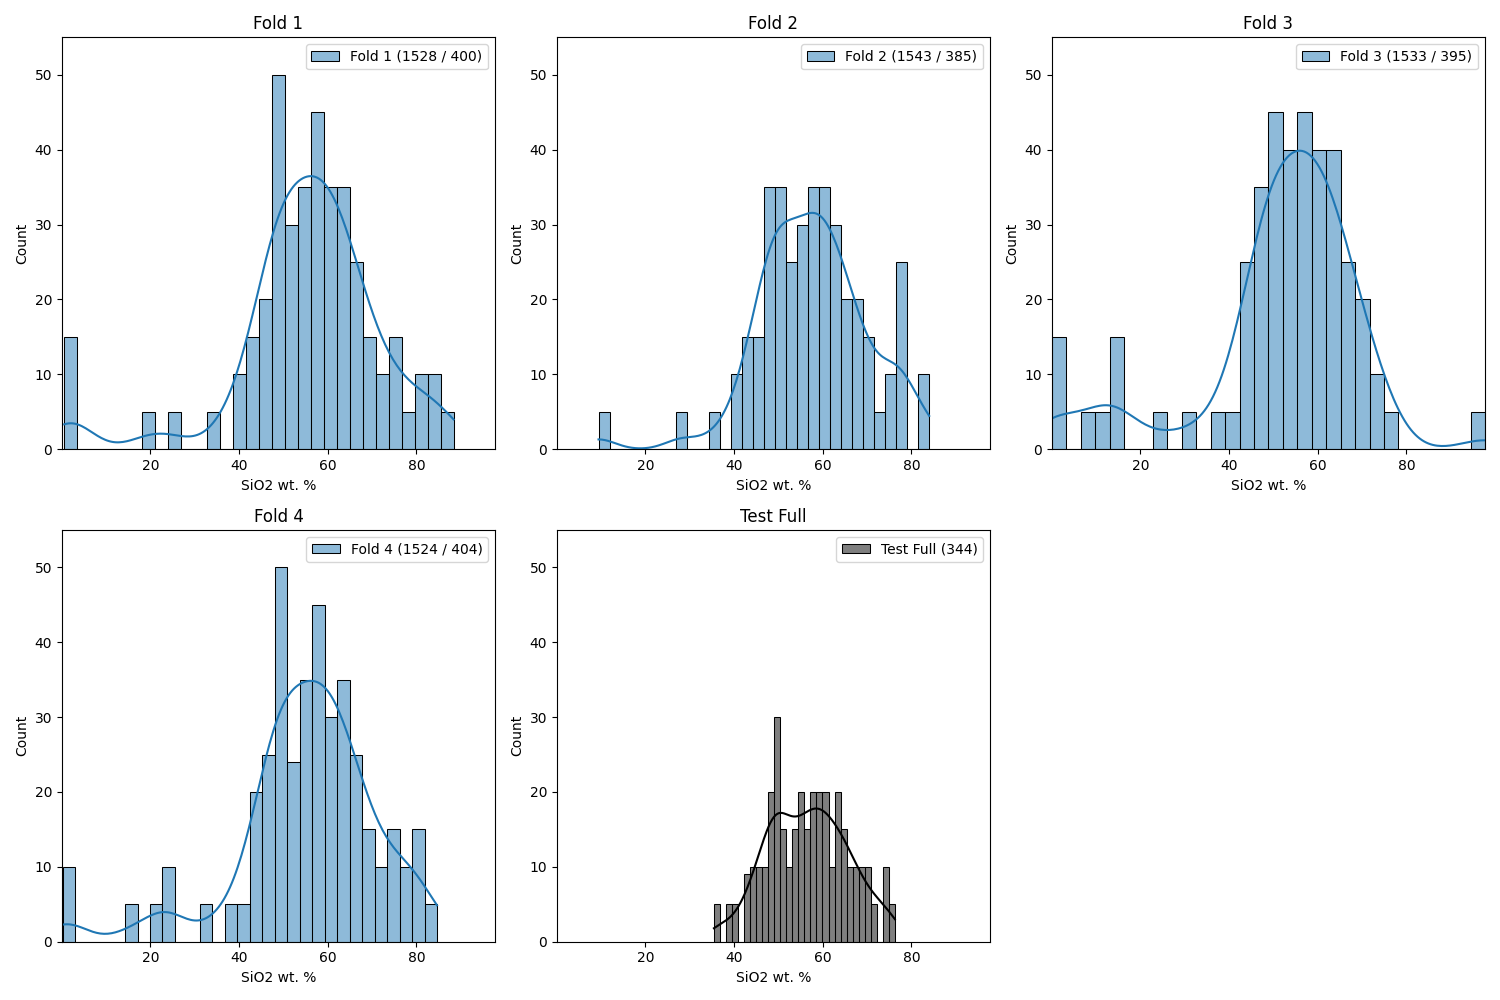
\includegraphics[width=\textwidth]{images/\oxide/histogram_grid_plot.png}
        \caption{Histogram and \gls{kde} of \ce{\oxide} distribution in each fold. The y-axis represents the count of samples per bin, and the x-axis represents \ce{\oxide} concentration. The notation in the legend indicates the amount of instances in the training/validation sets.}
        \label{fig:histogram_grid_plot_\oxide}
    \end{figure*}

    \begin{figure*}
        \centering
        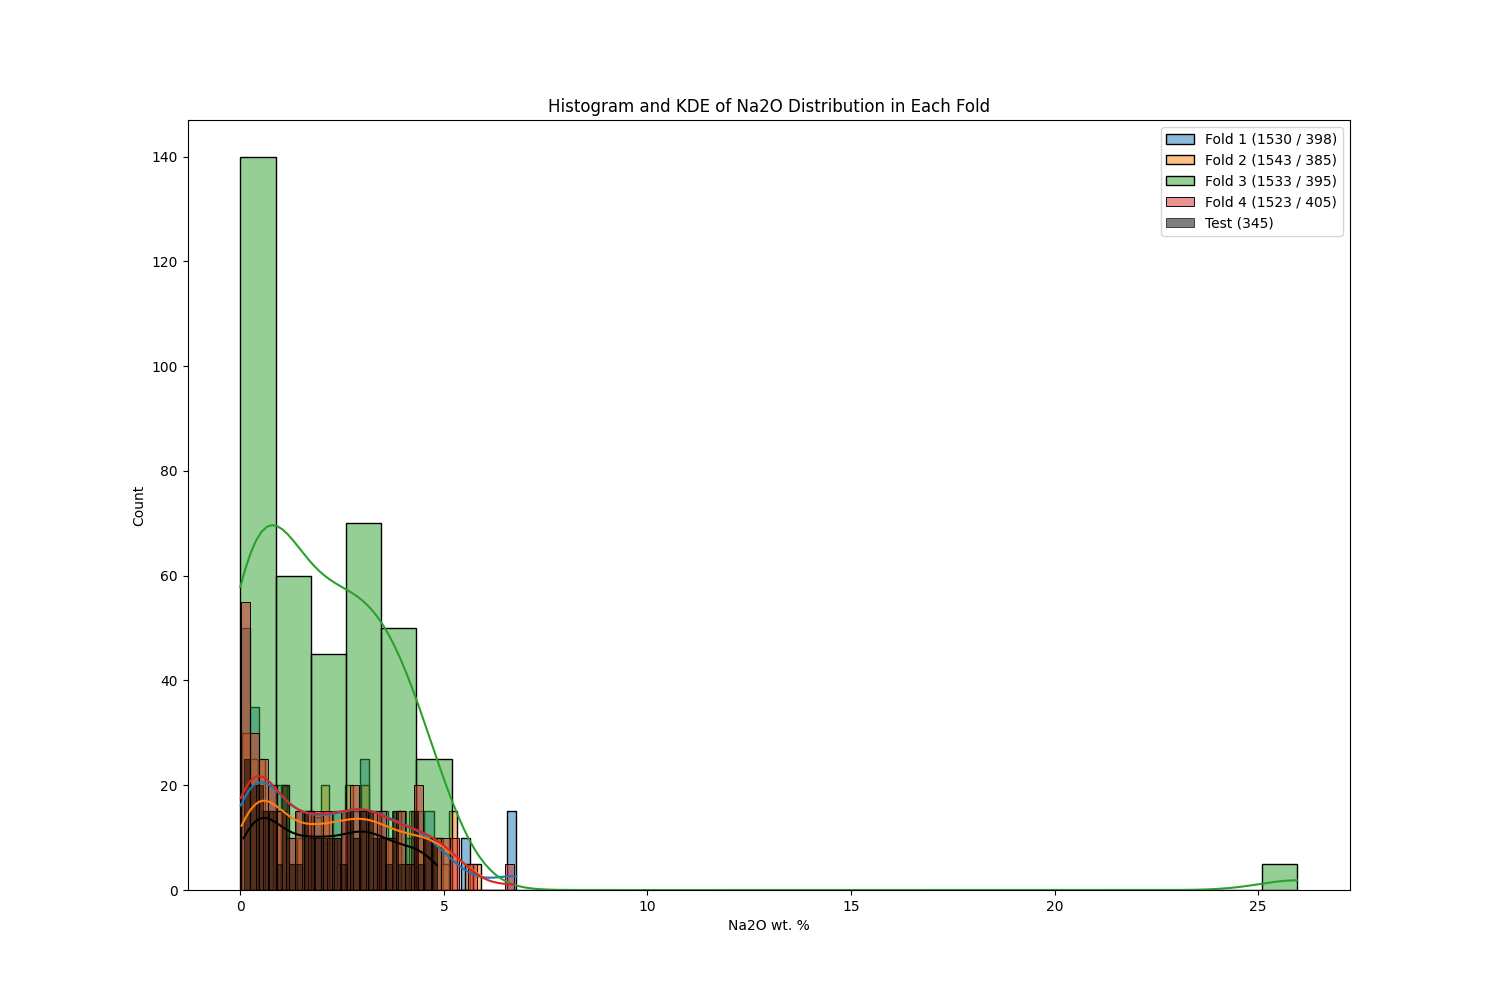
\includegraphics[width=\textwidth]{images/\oxide/histogram_kde_plot.png}
        \caption{Combined Histogram and \gls{kde} of \ce{\oxide} distribution in each fold. The y-axis represents the count of samples per bin, and the x-axis represents \ce{\oxide} concentration. The notation in the legend indicates the amount of instances in the training/validation sets.}
        \label{fig:histogram_kde_plot_\oxide}
    \end{figure*}

    \begin{figure*}
        \centering
        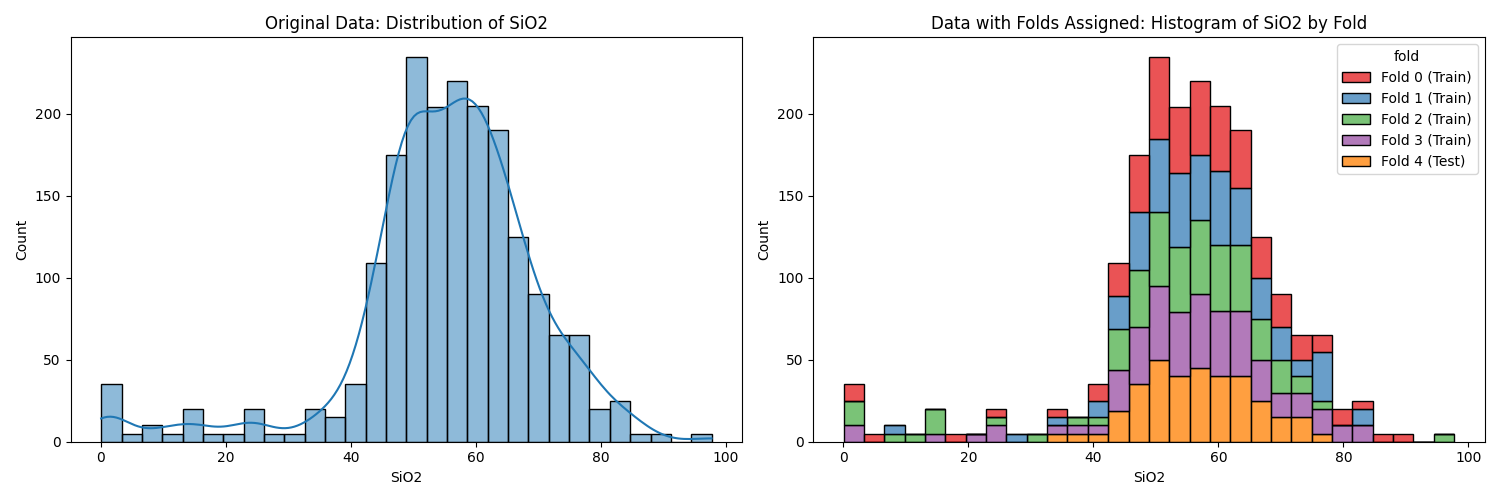
\includegraphics[width=\textwidth]{images/\oxide/original_and_post_fold.png}
        \caption{Distribution of \ce{\oxide} concentrations before and after fold assignment. The left plot shows the original distribution of \ce{\oxide}, while the right plot shows the distribution with folds assigned, color-coded to indicate the different folds.}
        \label{fig:original_and_post_fold_plot_\oxide}
    \end{figure*}

    \begin{figure*}
        \centering
        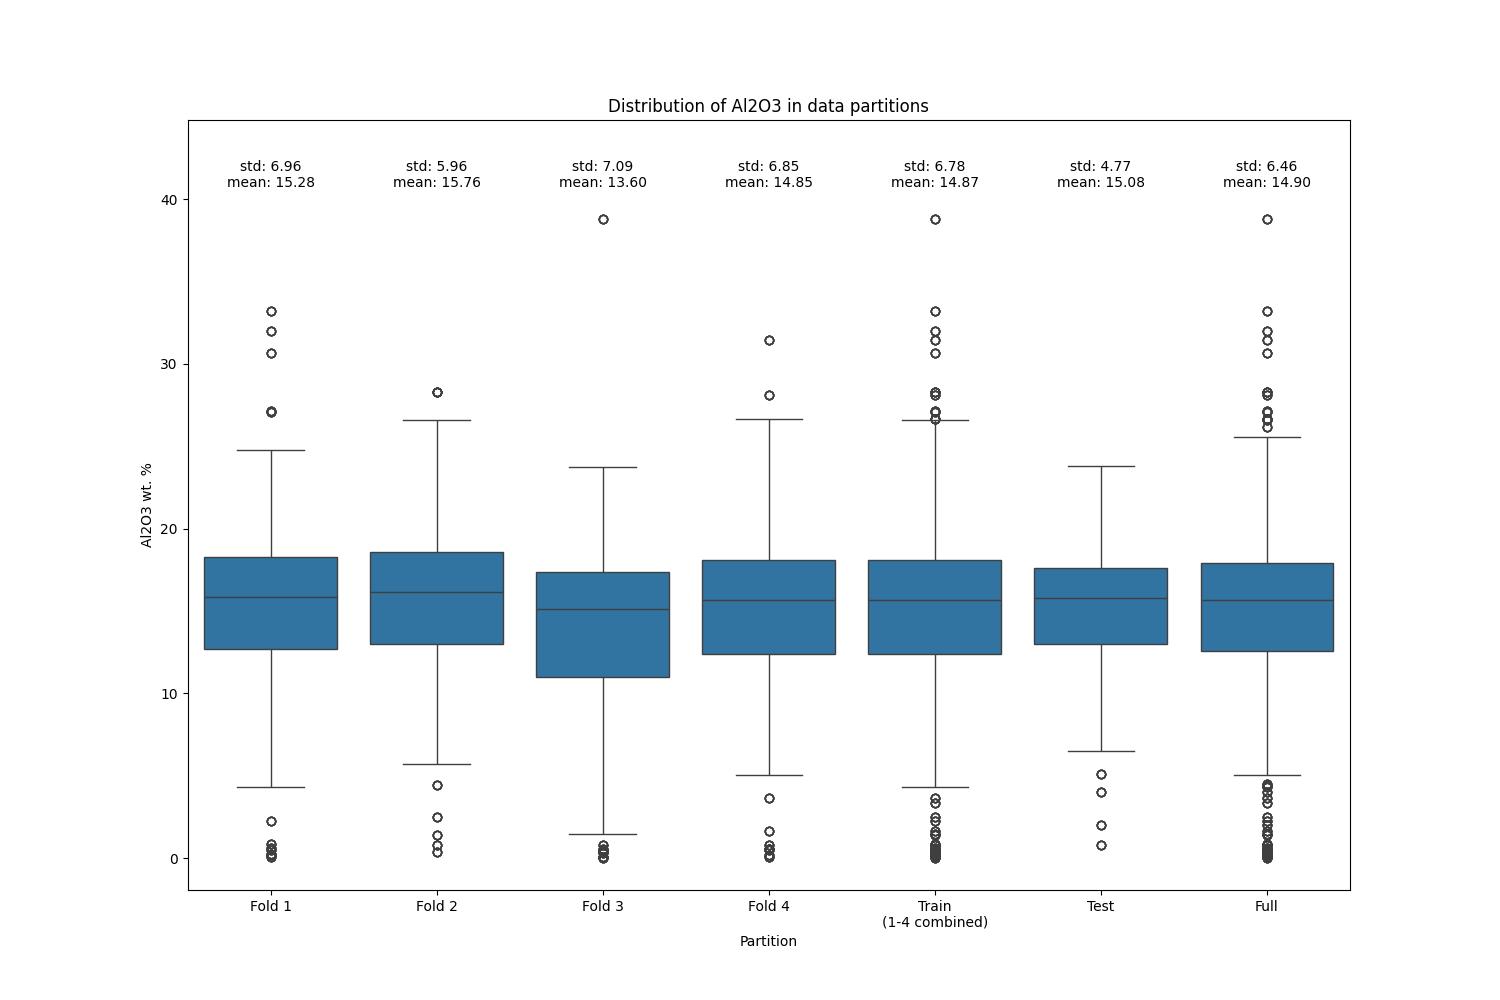
\includegraphics[width=\textwidth]{images/\oxide/distribution_plot.png}
        \caption{Distribution of \ce{\oxide} concentrations across cross-validation folds, training set, test set, and the entire dataset. The mean and standard deviation statistics for each partition are indicated figure.}
        \label{fig:distribution_plot_\oxide}
    \end{figure*}
}

\FloatBarrier

\subsection{Initial Experiment: Model Hyperparameters}\label{subsec:initial_experiment_hyperparameters}
\begin{table*}
\centering
\begin{tabular}{@{}llp{0.5\textwidth}@{}}
\toprule
\textbf{Model} & \textbf{Hyperparameter} & \textbf{Value} \\
\midrule
\multirow{3}{*}{\gls{pls}}
& \texttt{n\_components} & 34 \\
& \texttt{scale} & True \\
& \texttt{max\_iter} & 500 \\
\midrule
\multirow{6}{*}{\gls{svr}}
& \texttt{kernel} & poly \\
& \texttt{C} & 100 \\
& \texttt{epsilon} & 0.1 \\
& \texttt{gamma} & scale \\
& \texttt{degree} & 2 \\
& \texttt{coef0} & 1.0 \\
\midrule
\multirow{3}{*}{Ridge Regression}
& \texttt{alphas} & \{$10^{-4}$, $10^{-3}$, $10^{-2}$, $10^{-1}$, 1, 10, $10^2$, $10^3$\} \\
& \texttt{max\_iter} & 1000 \\
& \texttt{tol} & $10^{-4}$ \\
\midrule
\multirow{3}{*}{\gls{lasso}}
& \texttt{alphas} & \{$10^{-4}$, $10^{-3}$, $10^{-2}$, $10^{-1}$, 1, 10, $10^2$, $10^3$\} \\
& \texttt{max\_iter} & 1000 \\
& \texttt{tol} & $10^{-4}$ \\
\midrule
\multirow{4}{*}{\gls{enet}}
& \texttt{alphas} & \{$10^{-4}$, $10^{-3}$, $10^{-2}$, $10^{-1}$, 1, 10, $10^2$, $10^3$\} \\
& \texttt{l1\_ratio} & \{0.1, 0.5, 0.7, 0.9, 1.0\} \\
& \texttt{max\_iter} & 1000 \\
& \texttt{tol} & $10^{-4}$ \\
\midrule
\multirow{6}{*}{\gls{rf}}
& \texttt{n\_estimators} & 100 \\
& \texttt{max\_depth} & 10 \\
& \texttt{min\_samples\_split} & 2 \\
& \texttt{min\_samples\_leaf} & 1 \\
& \texttt{max\_features} & sqrt \\
& \texttt{random\_state} & 42 \\
\midrule
\multirow{5}{*}{\gls{etr}}
& \texttt{n\_estimators} & 100 \\
& \texttt{max\_depth} & 10 \\
& \texttt{min\_samples\_split} & 2 \\
& \texttt{min\_samples\_leaf} & 1 \\
& \texttt{random\_state} & 42 \\
\midrule
\end{tabular}
\caption{Explictly set hyperparameters for the \gls{pls}, \gls{svr}, ridge, \gls{lasso}, \gls{enet}, \gls{rf}, and \gls{etr} models. When not explicitly set, the default hyperparameters provided by the libraries listed in Section~\ref{sec:experimental_setup} are used.}
\label{tab:combined_hyperparameters}
\end{table*}

\FloatBarrier

\begin{table*}
\centering
\begin{tabular}{@{}llp{0.5\textwidth}@{}}
\toprule
\textbf{Model} & \textbf{Hyperparameter} & \textbf{Value} \\
\midrule
\multirow{14}{*}{\gls{gbr}}
& \texttt{n\_estimators} & 100 \\
& \texttt{max\_depth} & 3 \\
& \texttt{min\_samples\_split} & 2 \\
& \texttt{min\_samples\_leaf} & 1 \\
& \texttt{max\_features} & None \\
& \texttt{loss} & squared\_error \\
& \texttt{learning\_rate} & 0.1 \\
& \texttt{subsample} & 1.0 \\
& \texttt{criterion} & friedman\_mse \\
& \texttt{random\_state} & 42 \\
& \texttt{verbose} & 0 \\
& \texttt{validation\_fraction} & 0.1 \\
& \texttt{n\_iter\_no\_change} & None \\
& \texttt{tol} & $10^{-4}$ \\
& \texttt{ccp\_alpha} & 0.0 \\
\midrule
\gls{ngboost} & - & - \\
\midrule
\multirow{14}{*}{\gls{xgboost}}
& \texttt{max\_depth} & 4 \\
& \texttt{min\_child\_weight} & 5 \\
& \texttt{gamma} & 0.1 \\
& \texttt{subsample} & 0.7 \\
& \texttt{colsample\_bytree} & 0.5 \\
& \texttt{colsample\_bylevel} & 0.5 \\
& \texttt{colsample\_bynode} & 0.5 \\
& \texttt{lambda} & 1 \\
& \texttt{alpha} & 0.5 \\
& \texttt{learning\_rate} & 0.05 \\
& \texttt{n\_estimators} & 100 \\
& \texttt{objective} & reg:squarederror \\
& \texttt{eval\_metric} & rmse \\
\bottomrule
\end{tabular}
\caption{Explictly set hyperparameters for the \gls{gbr} and \gls{xgboost} models. When not explicitly set, the default hyperparameters provided by the libraries listed in Section~\ref{sec:experimental_setup} are used. The \gls{ngboost} model does not have any explicitly set hyperparameters.}
\label{tab:combined_hyperparameters}
\end{table*}

\FloatBarrier

\begin{table*}
  \centering
  \begin{tabular}{lll}
    \toprule
    \textbf{Layer} & \textbf{Output Shape} & \textbf{Hyperparameter} \\ \midrule
    Input & (\textit{input\_dim},) & - \\
    Dense & (1024,) & activation = ReLU \\
    Dropout & (1024,) & rate = 0.3 \\
    Dense & (512,) & activation = ReLU \\
    Dropout & (512,) & rate = 0.3 \\
    Dense & (256,) & activation = ReLU \\
    Dense & (128,) & activation = ReLU \\
    Output & (\textit{output\_dim},) & - \\
    \midrule
    \multicolumn{3}{l}{\textbf{Optimizer:} Adam} \\
    \multicolumn{3}{l}{\textbf{Learning Rate:} 0.001} \\
    \bottomrule
  \end{tabular}
  \caption{Summary of the Neural Network Architecture}
  \label{tab:nn_architecture}
\end{table*}

\begin{table*}
  \centering
  \begin{tabular}{lll}
    \toprule
    \textbf{Layer} & \textbf{Output Shape} & \textbf{Hyperparameter} \\ \midrule
    Input & (\textit{input\_dim},) & - \\
    Reshape & (48, 128, 1) & - \\
    Conv2D & (48, 128, 32) & filters = 32, kernel\_size = (3, 3), activation = ReLU, padding = 'same' \\
    BatchNormalization & (48, 128, 32) & - \\
    MaxPooling2D & (24, 64, 32) & pool\_size = (2, 2) \\ \midrule

    Conv2D & (24, 64, 32) & filters = 32, kernel\_size = (3, 3), activation = ReLU, padding = 'same' \\
    BatchNormalization & (24, 64, 32) & - \\
    MaxPooling2D & (12, 32, 32) & pool\_size = (2, 2) \\ \midrule

    Conv2D & (12, 32, 64) & filters = 64, kernel\_size = (3, 3), activation = ReLU, padding = 'same' \\
    BatchNormalization & (12, 32, 64) & - \\
    MaxPooling2D & (6, 16, 64) & pool\_size = (2, 2) \\ \midrule

    Conv2D & (6, 16, 128) & filters = 128, kernel\_size = (3, 3), activation = ReLU, padding = 'same' \\
    BatchNormalization & (6, 16, 128) & - \\
    MaxPooling2D & (3, 8, 128) & pool\_size = (2, 2) \\ \midrule

    Flatten & (3072,) & - \\
    Dense & (256,) & activation = ReLU \\
    Dropout & (256,) & rate = 0.5 \\
    Dense & (\textit{output\_dim},) & - \\
    Dense & (\textit{output\_dim},) & kernel\_regularizer = $L_2(0.01)$ \\ \midrule
    \multicolumn{3}{l}{\textbf{Optimizer:} Adam} \\
    \multicolumn{3}{l}{\textbf{Learning Rate:} 0.001} \\
    \bottomrule
  \end{tabular}
  \caption{Summary of the Convolutional Neural Network Architecture}
  \label{tab:cnn_architecture}
\end{table*}

\FloatBarrier

\subsection{Overview of best performing model configurations}\label{subsec:best_model_configurations}
\begin{table}[!htb]
\centering
\caption{Overview of model types for \ce{SiO2} oxide}
\begin{tabular}{llllllll}
\toprule
\ce{SiO2} & Model Type & Transformer Type & PCA Type & Scaler Type & \gls{rmsecv} & Std. dev. CV & \gls{rmsep} \\
\midrule
 & \texttt{pls} & \texttt{none} & \texttt{kernel\_pca} & \texttt{min\_max\_scaler} & 4.552 & 4.551 & 4.084 \\
 & \texttt{svr} & \texttt{none} & \texttt{none} & \texttt{min\_max\_scaler} & 4.592 & 4.588 & 3.533 \\
 & \texttt{gbr} & \texttt{none} & \texttt{none} & \texttt{norm3\_scaler} & 4.652 & 4.646 & 3.720 \\
 & \texttt{lasso} & \texttt{power\_transformer} & \texttt{pca} & \texttt{norm3\_scaler} & 4.737 & 4.738 & 4.248 \\
 & \texttt{xgboost} & \texttt{quantile\_transformer} & \texttt{none} & \texttt{norm3\_scaler} & 4.791 & 4.781 & 3.968 \\
 & \texttt{elasticnet} & \texttt{quantile\_transformer} & \texttt{none} & \texttt{norm3\_scaler} & 4.841 & 4.844 & 3.947 \\
 & \texttt{ngboost} & \texttt{power\_transformer} & \texttt{none} & \texttt{norm3\_scaler} & 4.860 & 4.851 & 4.148 \\
 & \texttt{ridge} & \texttt{power\_transformer} & \texttt{none} & \texttt{norm3\_scaler} & 4.940 & 4.938 & 3.816 \\
 & \texttt{extra\_trees} & \texttt{power\_transformer} & \texttt{none} & \texttt{norm3\_scaler} & 5.141 & 5.118 & 3.821 \\
 & \texttt{random\_forest} & \texttt{none} & \texttt{none} & \texttt{norm3\_scaler} & 5.204 & 5.192 & 3.788 \\
\bottomrule
\end{tabular}
\label{tab:SiO2_overview}
\end{table}

\begin{table*}
\centering
\begin{tabular}{llllllll}
\toprule
\ce{TiO2} & Model Type & Transformer Type & PCA Type & Scaler Type & \gls{rmsecv} & Std. dev. CV & \gls{rmsep} \\
\midrule
 & \texttt{svr} & \texttt{power\_transformer} & \texttt{none} & \texttt{norm3\_scaler} & 0.409 & 0.406 & 0.397 \\
 & \texttt{gbr} & \texttt{power\_transformer} & \texttt{none} & \texttt{norm3\_scaler} & 0.410 & 0.409 & 0.332 \\
 & \texttt{xgboost} & \texttt{none} & \texttt{none} & \texttt{robust\_scaler} & 0.411 & 0.410 & 0.317 \\
 & \texttt{random\_forest} & \texttt{quantile\_transformer} & \texttt{none} & \texttt{norm3\_scaler} & 0.422 & 0.421 & 0.334 \\
 & \texttt{elasticnet} & \texttt{none} & \texttt{none} & \texttt{robust\_scaler} & 0.423 & 0.423 & 0.351 \\
 & \texttt{extra\_trees} & \texttt{power\_transformer} & \texttt{none} & \texttt{standard\_scaler} & 0.426 & 0.426 & 0.338 \\
 & \texttt{ridge} & \texttt{none} & \texttt{none} & \texttt{min\_max\_scaler} & 0.428 & 0.427 & 0.359 \\
 & \texttt{lasso} & \texttt{power\_transformer} & \texttt{none} & \texttt{standard\_scaler} & 0.431 & 0.430 & 0.372 \\
 & \texttt{ngboost} & \texttt{none} & \texttt{none} & \texttt{robust\_scaler} & 0.431 & 0.431 & 0.355 \\
 & \texttt{pls} & \texttt{power\_transformer} & \texttt{kernel\_pca} & \texttt{robust\_scaler} & 0.441 & 0.441 & 0.411 \\
\bottomrule
\end{tabular}
\caption{Overview of model types for \ce{TiO2} oxide}
\label{tab:TiO2_overview}
\end{table*}

\begin{table*}
\centering
\begin{tabular}{llllllll}
\toprule
\ce{Al2O3} & Model Type & Transformer Type & PCA Type & Scaler Type & \gls{rmsecv} & Std. dev. CV & \gls{rmsep} \\
\midrule
 & \texttt{xgboost} & \texttt{power\_transformer} & \texttt{none} & \texttt{norm3\_scaler} & 2.075 & 2.067 & 1.740 \\
 & \texttt{gbr} & \texttt{power\_transformer} & \texttt{none} & \texttt{robust\_scaler} & 2.092 & 2.089 & 1.987 \\
 & \texttt{ngboost} & \texttt{power\_transformer} & \texttt{none} & \texttt{robust\_scaler} & 2.121 & 2.113 & 2.052 \\
 & \texttt{svr} & \texttt{quantile\_transformer} & \texttt{none} & \texttt{min\_max\_scaler} & 2.179 & 2.176 & 1.873 \\
 & \texttt{ridge} & \texttt{quantile\_transformer} & \texttt{none} & \texttt{norm3\_scaler} & 2.218 & 2.211 & 1.843 \\
 & \texttt{elasticnet} & \texttt{quantile\_transformer} & \texttt{none} & \texttt{norm3\_scaler} & 2.225 & 2.219 & 1.804 \\
 & \texttt{pls} & \texttt{quantile\_transformer} & \texttt{none} & \texttt{robust\_scaler} & 2.247 & 2.244 & 2.111 \\
 & \texttt{lasso} & \texttt{quantile\_transformer} & \texttt{none} & \texttt{norm3\_scaler} & 2.249 & 2.242 & 1.903 \\
 & \texttt{extra\_trees} & \texttt{power\_transformer} & \texttt{none} & \texttt{min\_max\_scaler} & 2.288 & 2.261 & 2.092 \\
 & \texttt{random\_forest} & \texttt{power\_transformer} & \texttt{none} & \texttt{max\_abs\_scaler} & 2.302 & 2.295 & 2.111 \\
\bottomrule
\end{tabular}
\caption{Overview of model types for \ce{Al2O3} oxide}
\label{tab:Al2O3_overview}
\end{table*}

\begin{table*}[htbp]
\centering
\begin{tabular}{llllllll}
\toprule
\ce{FeO_T} & Model Type & Transformer Type & PCA Type & Scaler Type & \gls{rmsecv} & Std. dev. CV & \gls{rmsep} \\
\midrule
 & \texttt{svr} & \texttt{quantile\_transformer} & \texttt{none} & \texttt{norm3\_scaler} & 2.242 & 2.243 & 1.803 \\
 & \texttt{pls} & \texttt{power\_transformer} & \texttt{none} & \texttt{standard\_scaler} & 2.701 & 2.669 & 2.063 \\
 & \texttt{ridge} & \texttt{quantile\_transformer} & \texttt{none} & \texttt{norm3\_scaler} & 2.707 & 2.687 & 1.878 \\
 & \texttt{gbr} & \texttt{power\_transformer} & \texttt{none} & \texttt{max\_abs\_scaler} & 2.749 & 2.750 & 1.793 \\
 & \texttt{xgboost} & \texttt{none} & \texttt{none} & \texttt{max\_abs\_scaler} & 2.749 & 2.743 & 1.622 \\
 & \texttt{elasticnet} & \texttt{power\_transformer} & \texttt{none} & \texttt{max\_abs\_scaler} & 2.862 & 2.831 & 1.773 \\
 & \texttt{lasso} & \texttt{quantile\_transformer} & \texttt{none} & \texttt{norm3\_scaler} & 2.875 & 2.862 & 1.842 \\
 & \texttt{extra\_trees} & \texttt{none} & \texttt{none} & \texttt{max\_abs\_scaler} & 2.900 & 2.903 & 1.870 \\
 & \texttt{ngboost} & \texttt{none} & \texttt{none} & \texttt{robust\_scaler} & 2.980 & 2.953 & 1.773 \\
 & \texttt{random\_forest} & \texttt{quantile\_transformer} & \texttt{none} & \texttt{norm3\_scaler} & 3.079 & 3.044 & 2.018 \\
\bottomrule
\end{tabular}
\caption{Overview of model types for \ce{FeO_T} oxide}
\label{tab:FeOT_overview}
\end{table*}

\begin{table*}[htbp]
\centering
\begin{tabular}{llllllll}
\toprule
\ce{MgO} & Model Type & Transformer Type & PCA Type & Scaler Type & \gls{rmsecv} & Std. dev. CV & \gls{rmsep} \\
\midrule
 & \texttt{svr} & \texttt{power\_transformer} & \texttt{none} & \texttt{robust\_scaler} & 1.322 & 1.321 & 0.791 \\
 & \texttt{pls} & \texttt{none} & \texttt{kernel\_pca} & \texttt{norm3\_scaler} & 1.327 & 1.321 & 0.993 \\
 & \texttt{ridge} & \texttt{power\_transformer} & \texttt{none} & \texttt{robust\_scaler} & 1.448 & 1.443 & 1.321 \\
 & \texttt{elasticnet} & \texttt{power\_transformer} & \texttt{none} & \texttt{robust\_scaler} & 1.466 & 1.462 & 1.630 \\
 & \texttt{gbr} & \texttt{quantile\_transformer} & \texttt{none} & \texttt{norm3\_scaler} & 1.468 & 1.464 & 0.880 \\
 & \texttt{extra\_trees} & \texttt{power\_transformer} & \texttt{none} & \texttt{norm3\_scaler} & 1.533 & 1.522 & 0.765 \\
 & \texttt{lasso} & \texttt{none} & \texttt{kernel\_pca} & \texttt{min\_max\_scaler} & 1.604 & 1.596 & 1.092 \\
 & \texttt{xgboost} & \texttt{none} & \texttt{none} & \texttt{norm3\_scaler} & 1.618 & 1.610 & 1.129 \\
 & \texttt{random\_forest} & \texttt{quantile\_transformer} & \texttt{none} & \texttt{norm3\_scaler} & 1.640 & 1.630 & 0.973 \\
 & \texttt{ngboost} & \texttt{none} & \texttt{none} & \texttt{norm3\_scaler} & 1.690 & 1.668 & 0.958 \\
\bottomrule
\end{tabular}
\caption{Overview of model types for \ce{MgO} oxide}
\label{tab:MgO_overview}
\end{table*}

\begin{table}[!htb]
\centering
\caption{Overview of model types for \ce{CaO} oxide}
\begin{tabular}{llllllll}
\toprule
\ce{CaO} & Model Type & Transformer Type & PCA Type & Scaler Type & \gls{rmsecv} & Std. dev. CV & \gls{rmsep} \\
\midrule
 & \texttt{svr} & \texttt{quantile\_transformer} & \texttt{none} & \texttt{min\_max\_scaler} & 1.193 & 1.192 & 1.600 \\
 & \texttt{pls} & \texttt{quantile\_transformer} & \texttt{none} & \texttt{max\_abs\_scaler} & 1.270 & 1.263 & 1.768 \\
 & \texttt{gbr} & \texttt{quantile\_transformer} & \texttt{none} & \texttt{norm3\_scaler} & 1.281 & 1.280 & 1.793 \\
 & \texttt{extra\_trees} & \texttt{none} & \texttt{none} & \texttt{norm3\_scaler} & 1.308 & 1.309 & 1.829 \\
 & \texttt{xgboost} & \texttt{power\_transformer} & \texttt{none} & \texttt{norm3\_scaler} & 1.363 & 1.361 & 1.913 \\
 & \texttt{elasticnet} & \texttt{quantile\_transformer} & \texttt{none} & \texttt{norm3\_scaler} & 1.384 & 1.377 & 1.634 \\
 & \texttt{ridge} & \texttt{quantile\_transformer} & \texttt{none} & \texttt{norm3\_scaler} & 1.406 & 1.400 & 1.623 \\
 & \texttt{random\_forest} & \texttt{none} & \texttt{none} & \texttt{norm3\_scaler} & 1.439 & 1.435 & 1.737 \\
 & \texttt{ngboost} & \texttt{none} & \texttt{none} & \texttt{robust\_scaler} & 1.488 & 1.481 & 1.920 \\
 & \texttt{lasso} & \texttt{power\_transformer} & \texttt{none} & \texttt{min\_max\_scaler} & 1.529 & 1.514 & 1.684 \\
\bottomrule
\end{tabular}
\label{tab:CaO_overview}
\end{table}

\begin{table*}
\centering
\begin{tabular}{llllllll}
\toprule
\ce{Na2O} & Model Type & Transformer Type & PCA Type & Scaler Type & \gls{rmsecv} & Std. dev. CV & \gls{rmsep} \\
\midrule
 & \texttt{svr} & \texttt{power\_transformer} & \texttt{none} & \texttt{norm3\_scaler} & 0.777 & 0.775 & 0.393 \\
 & \texttt{pls} & \texttt{power\_transformer} & \texttt{none} & \texttt{norm3\_scaler} & 0.845 & 0.842 & 0.561 \\
 & \texttt{gbr} & \texttt{quantile\_transformer} & \texttt{none} & \texttt{norm3\_scaler} & 0.904 & 0.895 & 0.374 \\
 & \texttt{xgboost} & \texttt{quantile\_transformer} & \texttt{none} & \texttt{max\_abs\_scaler} & 0.952 & 0.943 & 0.431 \\
 & \texttt{extra\_trees} & \texttt{quantile\_transformer} & \texttt{none} & \texttt{norm3\_scaler} & 0.965 & 0.953 & 0.479 \\
 & \texttt{elasticnet} & \texttt{quantile\_transformer} & \texttt{none} & \texttt{standard\_scaler} & 0.994 & 0.990 & 0.504 \\
 & \texttt{lasso} & \texttt{quantile\_transformer} & \texttt{none} & \texttt{max\_abs\_scaler} & 0.995 & 0.991 & 0.507 \\
 & \texttt{ngboost} & \texttt{quantile\_transformer} & \texttt{none} & \texttt{norm3\_scaler} & 1.000 & 0.993 & 0.443 \\
 & \texttt{random\_forest} & \texttt{quantile\_transformer} & \texttt{none} & \texttt{norm3\_scaler} & 1.002 & 0.995 & 0.470 \\
 & \texttt{ridge} & \texttt{quantile\_transformer} & \texttt{none} & \texttt{norm3\_scaler} & 1.011 & 1.001 & 0.467 \\
\bottomrule
\end{tabular}
\caption{Overview of model types for \ce{Na2O} oxide}
\label{tab:Na2O_overview}
\end{table*}

\begin{table*}
\centering
\begin{tabular}{llllllll}
\toprule
\ce{K2O} & Model Type & Transformer Type & PCA Type & Scaler Type & \gls{rmsecv} & Std. dev. CV & \gls{rmsep} \\
\midrule
 & \texttt{pls} & \texttt{none} & \texttt{none} & \texttt{norm3\_scaler} & 0.587 & 0.586 & 0.724 \\
 & \texttt{gbr} & \texttt{quantile\_transformer} & \texttt{none} & \texttt{min\_max\_scaler} & 0.590 & 0.587 & 0.423 \\
 & \texttt{svr} & \texttt{quantile\_transformer} & \texttt{none} & \texttt{norm3\_scaler} & 0.593 & 0.593 & 0.594 \\
 & \texttt{xgboost} & \texttt{power\_transformer} & \texttt{none} & \texttt{standard\_scaler} & 0.600 & 0.599 & 0.455 \\
 & \texttt{elasticnet} & \texttt{power\_transformer} & \texttt{none} & \texttt{robust\_scaler} & 0.602 & 0.602 & 0.650 \\
 & \texttt{ngboost} & \texttt{quantile\_transformer} & \texttt{none} & \texttt{max\_abs\_scaler} & 0.602 & 0.600 & 0.420 \\
 & \texttt{lasso} & \texttt{power\_transformer} & \texttt{none} & \texttt{norm3\_scaler} & 0.607 & 0.606 & 0.624 \\
 & \texttt{ridge} & \texttt{power\_transformer} & \texttt{none} & \texttt{norm3\_scaler} & 0.611 & 0.611 & 0.629 \\
 & \texttt{random\_forest} & \texttt{power\_transformer} & \texttt{none} & \texttt{norm3\_scaler} & 0.675 & 0.669 & 0.515 \\
 & \texttt{extra\_trees} & \texttt{power\_transformer} & \texttt{none} & \texttt{robust\_scaler} & 0.714 & 0.709 & 0.464 \\
\bottomrule
\end{tabular}
\caption{Overview of model types for \ce{K2O} oxide}
\label{tab:K2O_overview}
\end{table*}


\FloatBarrier

\subsection{Stacking Ensemble 1:1 Plots}\label{subsec:1_1_plots}
\begin{figure*}
    \centering
    \resizebox{0.75\textwidth}{!}{
        \begin{tabular}{cc}
            \begin{subfigure}{0.5\textwidth}
                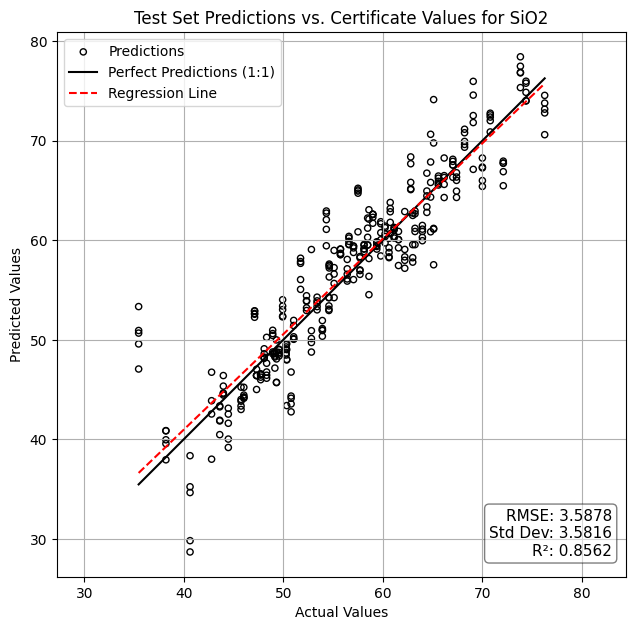
\includegraphics[width=\textwidth]{images/one_to_one/elasticnet/SiO2.png}
            \end{subfigure} & \hspace{3cm}
            \begin{subfigure}{0.5\textwidth}
                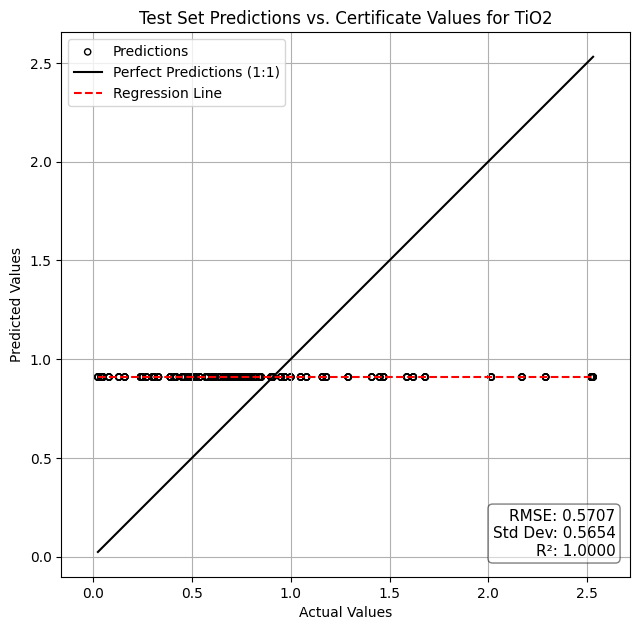
\includegraphics[width=\textwidth]{images/one_to_one/elasticnet/TiO2.png}
            \end{subfigure} \\
            \begin{subfigure}{0.5\textwidth}
                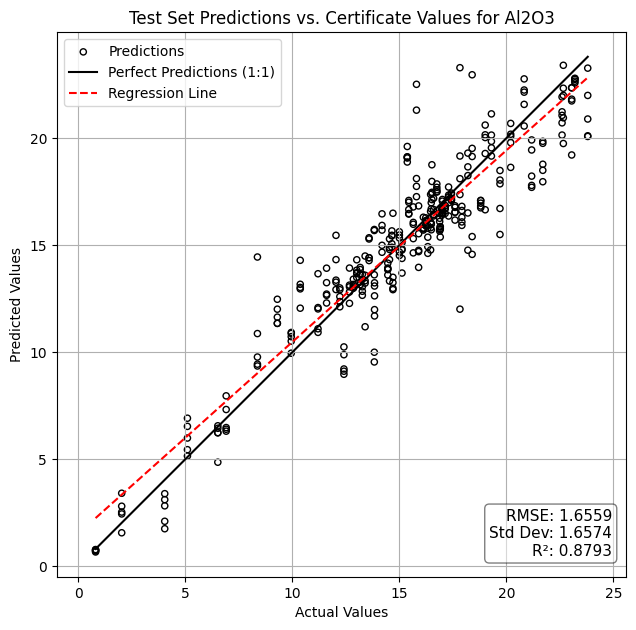
\includegraphics[width=\textwidth]{images/one_to_one/elasticnet/Al2O3.png}
            \end{subfigure} & \hspace{3cm}
            \begin{subfigure}{0.5\textwidth}
                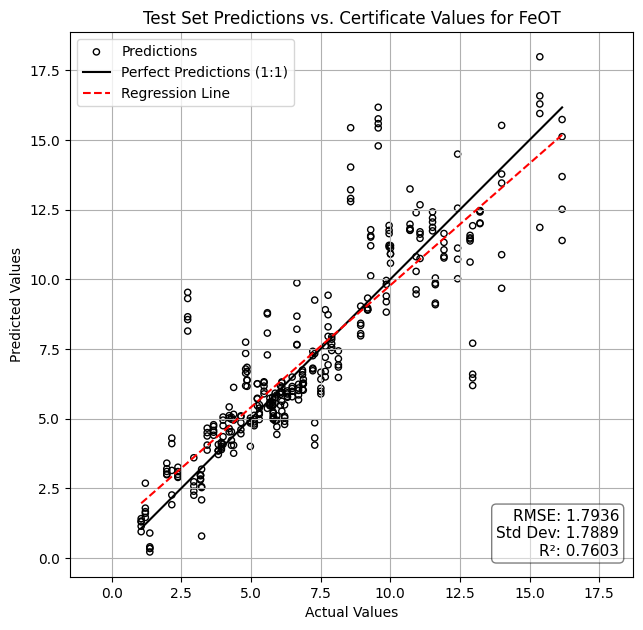
\includegraphics[width=\textwidth]{images/one_to_one/elasticnet/FeOT.png}
            \end{subfigure} \\
            \begin{subfigure}{0.5\textwidth}
                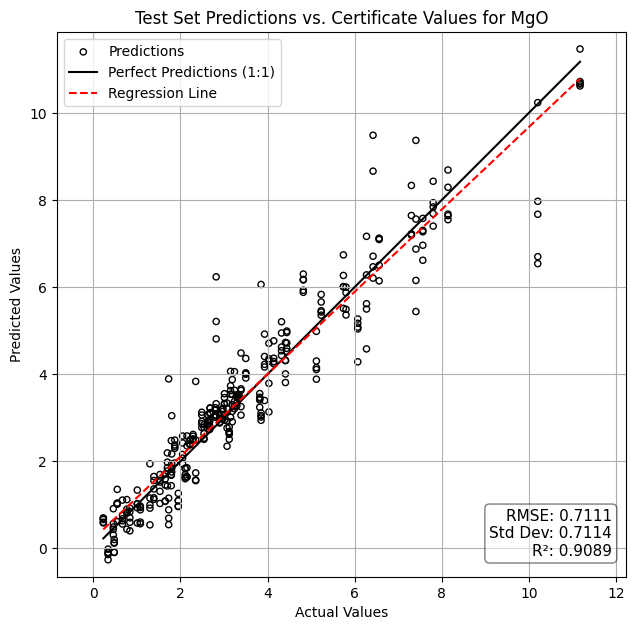
\includegraphics[width=\textwidth]{images/one_to_one/elasticnet/MgO.png}
            \end{subfigure} & \hspace{3cm}
            \begin{subfigure}{0.5\textwidth}
                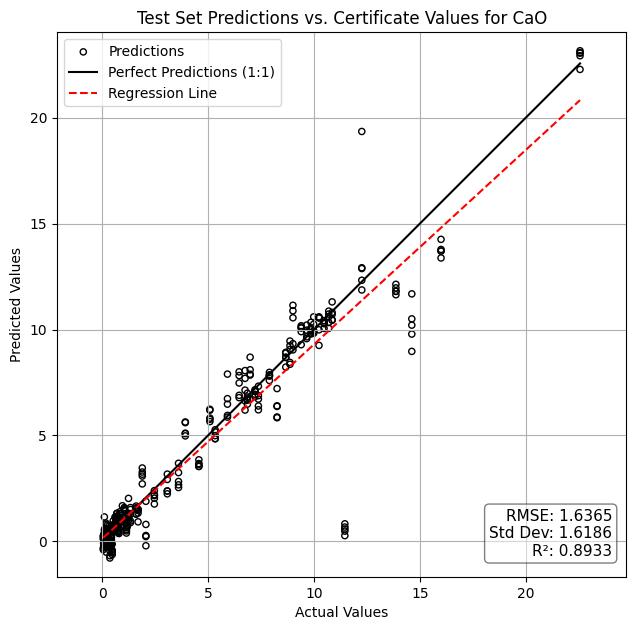
\includegraphics[width=\textwidth]{images/one_to_one/elasticnet/CaO.png}
            \end{subfigure} \\
            \begin{subfigure}{0.5\textwidth}
                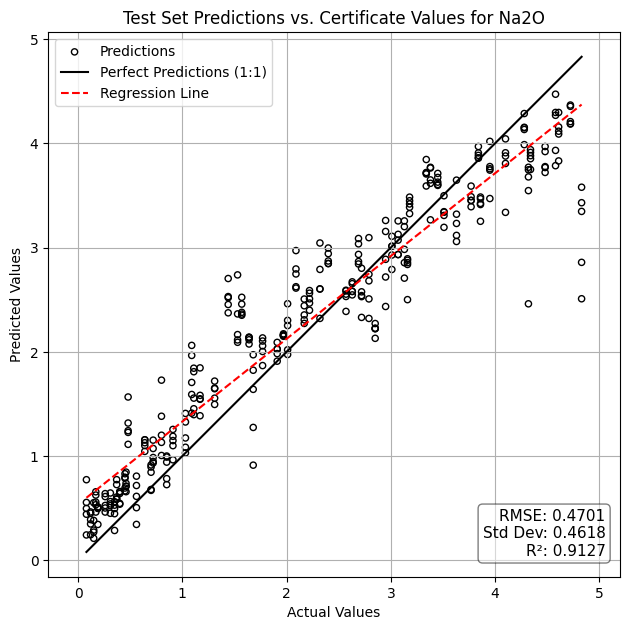
\includegraphics[width=\textwidth]{images/one_to_one/elasticnet/Na2O.png}
            \end{subfigure} & \hspace{3cm}
            \begin{subfigure}{0.5\textwidth}
                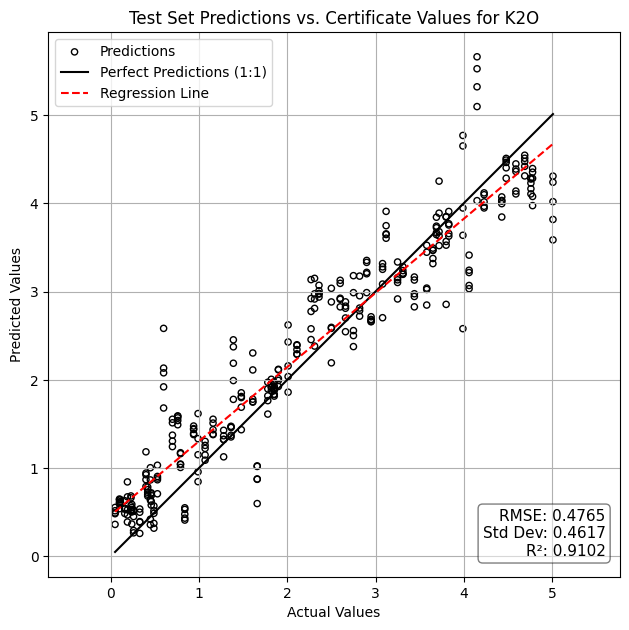
\includegraphics[width=\textwidth]{images/one_to_one/elasticnet/K2O.png}
            \end{subfigure}
        \end{tabular}
    }
    \caption{One-to-one plots for the stacking ensemble model with the \gls{enet} as the meta-learner with $\alpha = 1$}
    \label{fig:elasticnet_one_to_one}
\end{figure*}

\begin{figure*}
    \centering
    \resizebox{0.75\textwidth}{!}{
        \begin{tabular}{cc}
            \begin{subfigure}{0.5\textwidth}
                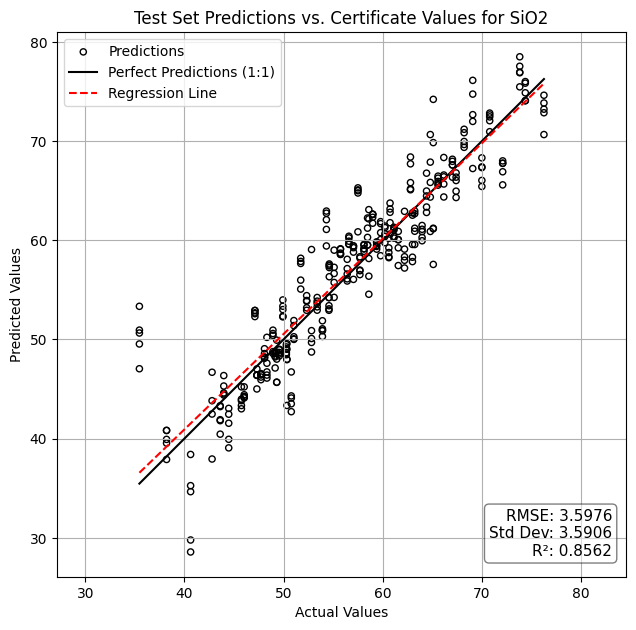
\includegraphics[width=\textwidth]{images/one_to_one/enetalpha01/SiO2.png}
            \end{subfigure} & \hspace{3cm}
            \begin{subfigure}{0.5\textwidth}
                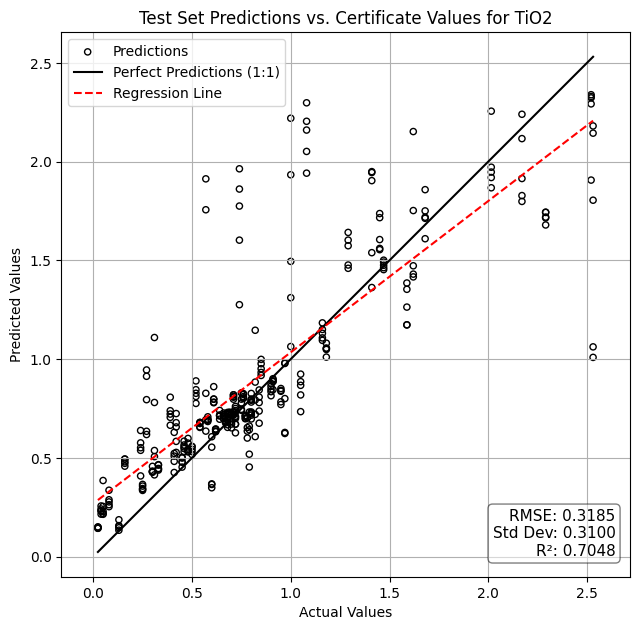
\includegraphics[width=\textwidth]{images/one_to_one/enetalpha01/TiO2.png}
            \end{subfigure} \\
            \begin{subfigure}{0.5\textwidth}
                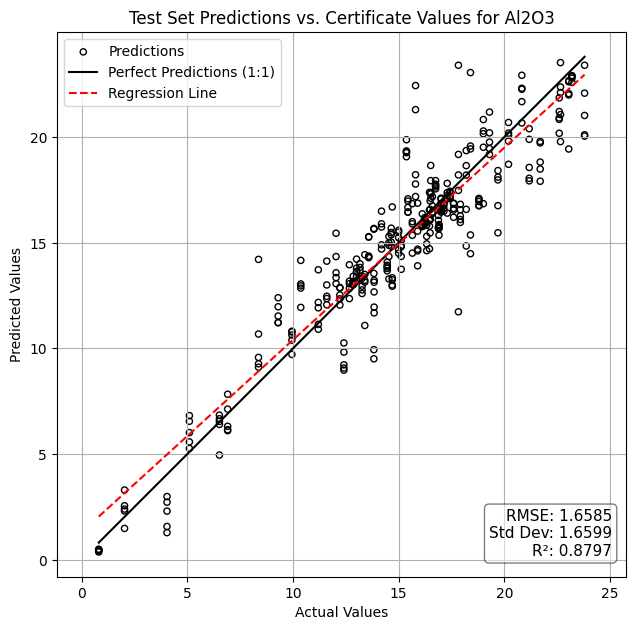
\includegraphics[width=\textwidth]{images/one_to_one/enetalpha01/Al2O3.png}
            \end{subfigure} & \hspace{3cm}
            \begin{subfigure}{0.5\textwidth}
                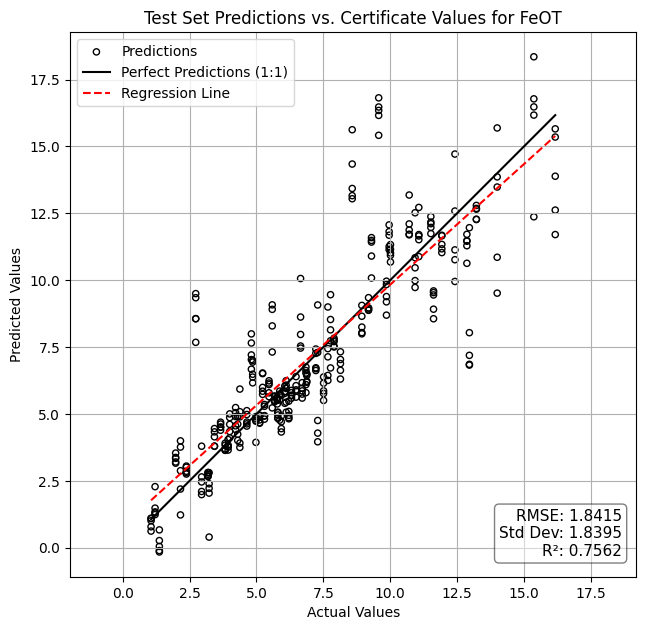
\includegraphics[width=\textwidth]{images/one_to_one/enetalpha01/FeOT.png}
            \end{subfigure} \\
            \begin{subfigure}{0.5\textwidth}
                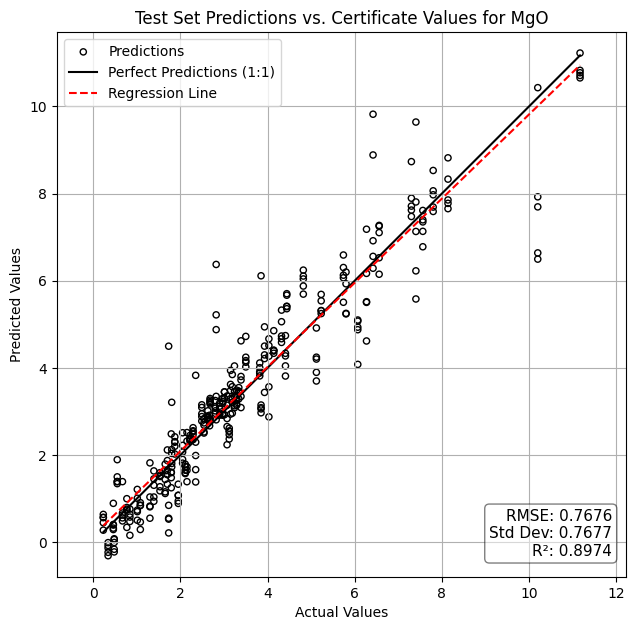
\includegraphics[width=\textwidth]{images/one_to_one/enetalpha01/MgO.png}
            \end{subfigure} & \hspace{3cm}
            \begin{subfigure}{0.5\textwidth}
                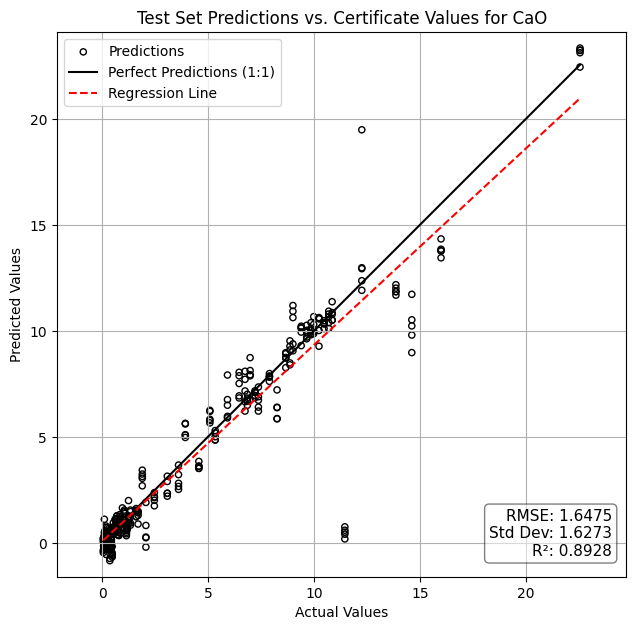
\includegraphics[width=\textwidth]{images/one_to_one/enetalpha01/CaO.png}
            \end{subfigure} \\
            \begin{subfigure}{0.5\textwidth}
                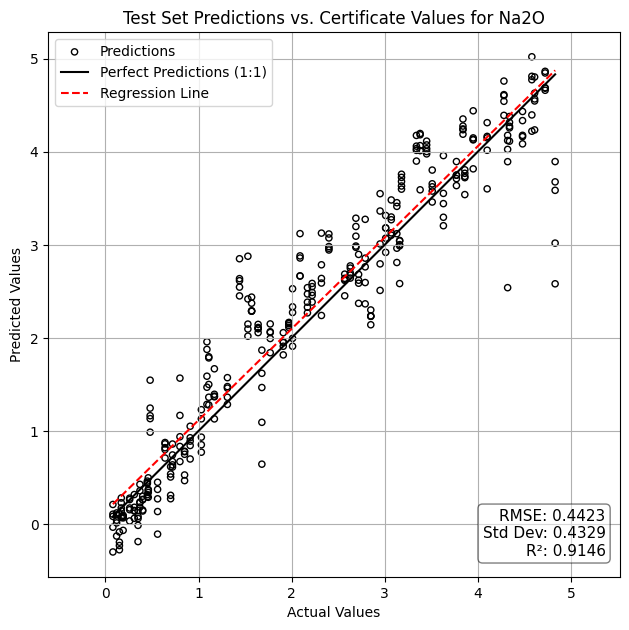
\includegraphics[width=\textwidth]{images/one_to_one/enetalpha01/Na2O.png}
            \end{subfigure} & \hspace{3cm}
            \begin{subfigure}{0.5\textwidth}
                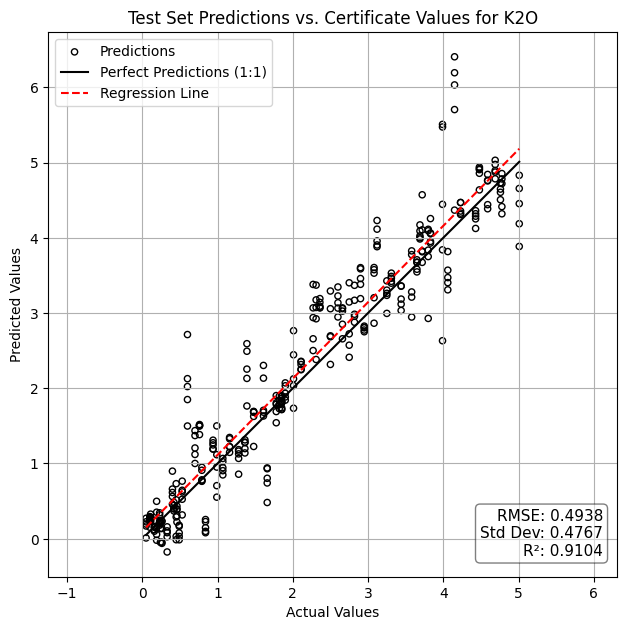
\includegraphics[width=\textwidth]{images/one_to_one/enetalpha01/K2O.png}
            \end{subfigure}
        \end{tabular}
    }
    \caption{One-to-one plots for the stacking ensemble model with the \gls{enet} as the meta-learner with $\alpha = 0.1$.}
    \label{fig:enetalpha01_one_to_one}
\end{figure*}

\begin{figure*}
    \centering
    \resizebox{0.75\textwidth}{!}{
        \begin{tabular}{cc}
            \begin{subfigure}{0.5\textwidth}
                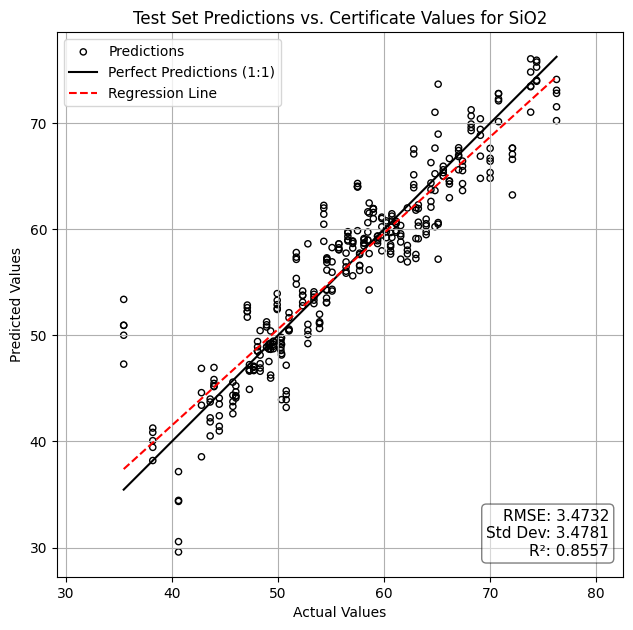
\includegraphics[width=\textwidth]{images/one_to_one/svr/SiO2.png}
            \end{subfigure} & \hspace{3cm}
            \begin{subfigure}{0.5\textwidth}
                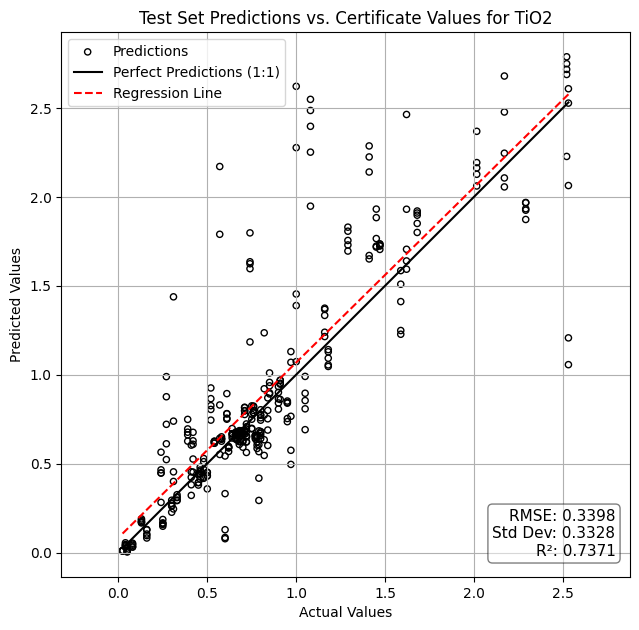
\includegraphics[width=\textwidth]{images/one_to_one/svr/TiO2.png}
            \end{subfigure} \\
            \begin{subfigure}{0.5\textwidth}
                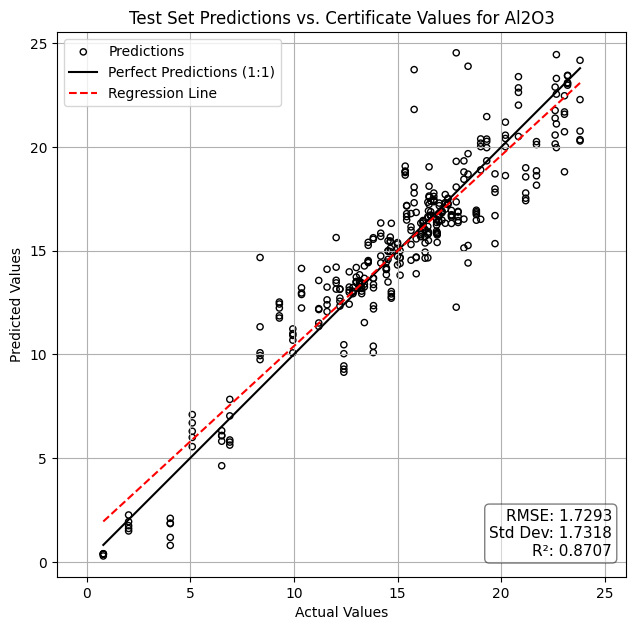
\includegraphics[width=\textwidth]{images/one_to_one/svr/Al2O3.png}
            \end{subfigure} & \hspace{3cm}
            \begin{subfigure}{0.5\textwidth}
                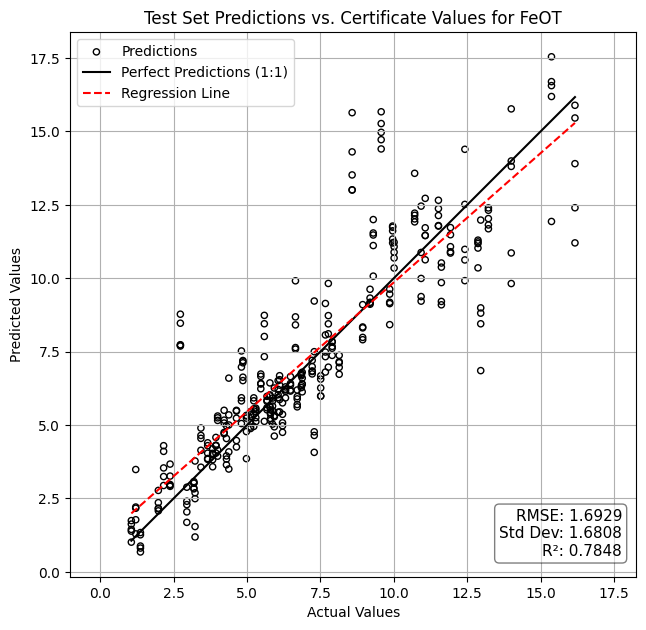
\includegraphics[width=\textwidth]{images/one_to_one/svr/FeOT.png}
            \end{subfigure} \\
            \begin{subfigure}{0.5\textwidth}
                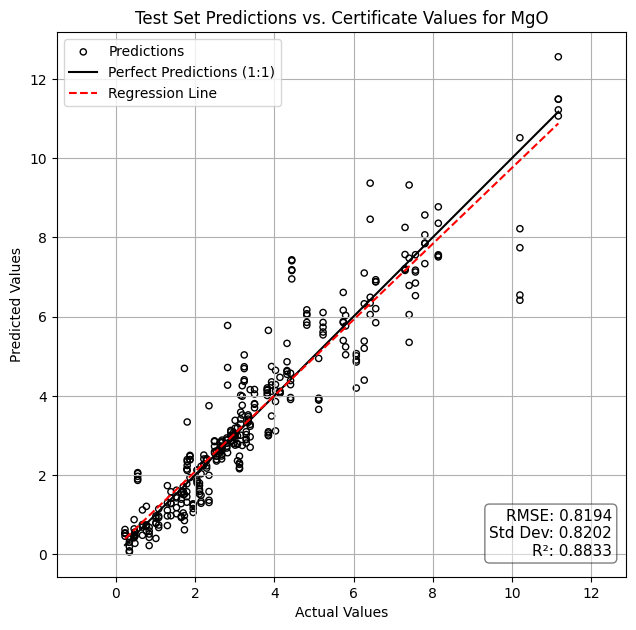
\includegraphics[width=\textwidth]{images/one_to_one/svr/MgO.png}
            \end{subfigure} & \hspace{3cm}
            \begin{subfigure}{0.5\textwidth}
                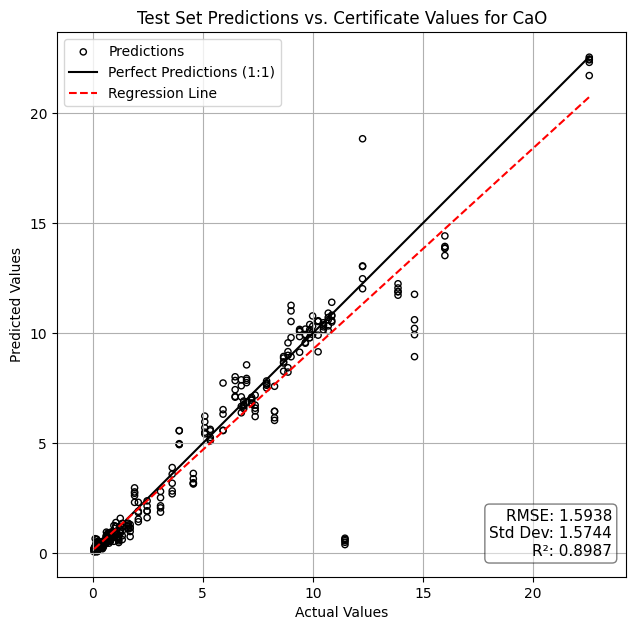
\includegraphics[width=\textwidth]{images/one_to_one/svr/CaO.png}
            \end{subfigure} \\
            \begin{subfigure}{0.5\textwidth}
                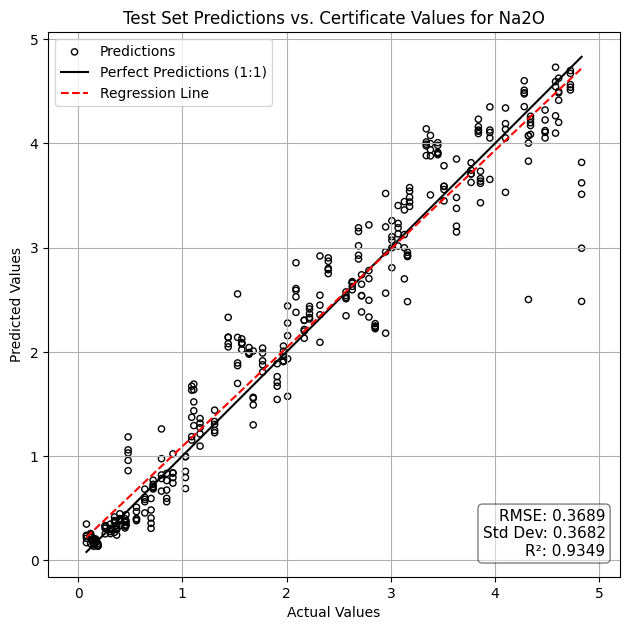
\includegraphics[width=\textwidth]{images/one_to_one/svr/Na2O.png}
            \end{subfigure} & \hspace{3cm}
            \begin{subfigure}{0.5\textwidth}
                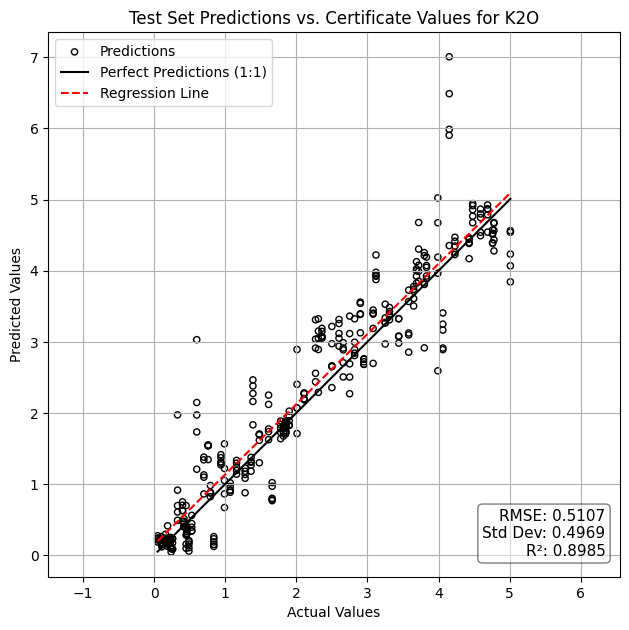
\includegraphics[width=\textwidth]{images/one_to_one/svr/K2O.png}
            \end{subfigure}
        \end{tabular}
    }
    \caption{One-to-one plots for the stacking ensemble model with the \gls{svr} as the meta-learner}
    \label{fig:svr_one_to_one}
\end{figure*}
